% Options for packages loaded elsewhere
\PassOptionsToPackage{unicode}{hyperref}
\PassOptionsToPackage{hyphens}{url}
%
\documentclass{article}
\usepackage{lmodern}
\usepackage{amssymb,amsmath}
\usepackage{ifxetex,ifluatex}
\ifnum 0\ifxetex 1\fi\ifluatex 1\fi=0 % if pdftex
  \usepackage[T1]{fontenc}
  \usepackage[utf8]{inputenc}
  \usepackage{textcomp} % provide euro and other symbols
\else % if luatex or xetex
  \usepackage{unicode-math}
  \defaultfontfeatures{Scale=MatchLowercase}
  \defaultfontfeatures[\rmfamily]{Ligatures=TeX,Scale=1}
\fi
% Use upquote if available, for straight quotes in verbatim environments
\IfFileExists{upquote.sty}{\usepackage{upquote}}{}
\IfFileExists{microtype.sty}{% use microtype if available
  \usepackage[]{microtype}
  \UseMicrotypeSet[protrusion]{basicmath} % disable protrusion for tt fonts
}{}
\makeatletter
\@ifundefined{KOMAClassName}{% if non-KOMA class
  \IfFileExists{parskip.sty}{%
    \usepackage{parskip}
  }{% else
    \setlength{\parindent}{0pt}
    \setlength{\parskip}{6pt plus 2pt minus 1pt}}
}{% if KOMA class
  \KOMAoptions{parskip=half}}
\makeatother
\usepackage{xcolor}
\IfFileExists{xurl.sty}{\usepackage{xurl}}{} % add URL line breaks if available
\IfFileExists{bookmark.sty}{\usepackage{bookmark}}{\usepackage{hyperref}}
\hypersetup{
  pdftitle={2020 Project},
  pdfauthor={Ryan G - 17805315},
  hidelinks,
  pdfcreator={LaTeX via pandoc}}
\urlstyle{same} % disable monospaced font for URLs
\usepackage{listings}
\newcommand{\passthrough}[1]{#1}
\lstset{defaultdialect=[5.3]Lua}
\lstset{defaultdialect=[x86masm]Assembler}
\usepackage{longtable,booktabs}
% Correct order of tables after \paragraph or \subparagraph
\usepackage{etoolbox}
\makeatletter
\patchcmd\longtable{\par}{\if@noskipsec\mbox{}\fi\par}{}{}
\makeatother
% Allow footnotes in longtable head/foot
\IfFileExists{footnotehyper.sty}{\usepackage{footnotehyper}}{\usepackage{footnote}}
\makesavenoteenv{longtable}
\usepackage{graphicx}
\makeatletter
\def\maxwidth{\ifdim\Gin@nat@width>\linewidth\linewidth\else\Gin@nat@width\fi}
\def\maxheight{\ifdim\Gin@nat@height>\textheight\textheight\else\Gin@nat@height\fi}
\makeatother
% Scale images if necessary, so that they will not overflow the page
% margins by default, and it is still possible to overwrite the defaults
% using explicit options in \includegraphics[width, height, ...]{}
\setkeys{Gin}{width=\maxwidth,height=\maxheight,keepaspectratio}
% Set default figure placement to htbp
\makeatletter
\def\fps@figure{htbp}
\makeatother
\setlength{\emergencystretch}{3em} % prevent overfull lines
\providecommand{\tightlist}{%
  \setlength{\itemsep}{0pt}\setlength{\parskip}{0pt}}
% \setcounter{secnumdepth}{-\maxdimen} % remove section numbering
\ProvidesPackage{ScreenStyle}

% I should split this up into a style sheet and a preamble.
% Inside a style sheet, the correct behaviour is to use RequirePackage rather
% than RequirePackage

% * Packages
% ** General
%\RequirePackage{~/Dropbox/profiles/Templates/LaTeX/texnotePreamble.sty}
\RequirePackage[utf8]{inputenc}
%\RequirePackage{fontspec} %More support for fonts in XeTeX
%\RequirePackage[Latin,Greek,Emoticons]{ucharclasses}
%\RequirePackage[framemethod=tikz]{mdframed}
\RequirePackage{pgfplots}
\RequirePackage{comment}
\RequirePackage{import} %This is allows relative directories
\RequirePackage{tikz, pstricks}
%\usetikzlibrary{calc}
%\RequirePackage{chngcntr}
\RequirePackage[T1]{fontenc}
%\RequirePackage{extsizes} % More Font Sizes
\RequirePackage[utf8]{inputenc}
\RequirePackage{sectsty} %Need it for underlining Sections
\RequirePackage{lmodern}
\RequirePackage{enumitem}
\RequirePackage{ifxetex,ifluatex} % This doesn't work with org-mode
\RequirePackage{lipsum}
\RequirePackage[T1]{fontenc}
\RequirePackage[utf8]{inputenc}
\RequirePackage[margin=1in]{geometry}
\addtolength{\skip\footins}{2pc plus 5pt} %Add whitespace before footnotes`
%\RequirePackage{tgadventor}
% Titlesec is incompatible with org-mode
% ** Styles
%\RequirePackage{titlesec} % Section Colours
% *** Colours
%\RequirePackage[svgnames, x11names, dvipsnames]{xcolor} %This is included with mdframed
% ** Graphics

\RequirePackage{graphicx}
% ** AmsMath
\RequirePackage{amsmath, amssymb, amsthm}

%Use this to put it in TOC
%\printbibliography[heading=bibintoc, title={Whole bibliography}]
%\printbibliography[heading=subbibintoc,type=article,title={Articles only}]
% ** Bibliography
\RequirePackage[citestyle=numeric, bibstyle=numeric,hyperref=true,backref=true, maxcitenames=3,url=true,backend=biber,natbib=true]{biblatex}
\addbibresource{/home/ryan/Dropbox/Studies/Papers/references.bib}
\AtEndDocument{\printbibliography}

%Use this to put it in TOC
%\printbibliography[heading=bibintoc, title={Whole bibliography}]
%\printbibliography[heading=subbibintoc,type=article,title={Articles only}]
% ** Hyperref (Last)

%Hyperlinks----------------must load last ---------------
\RequirePackage{bibentry}
\RequirePackage{hyperref}
\hypersetup{
	colorlinks,
	citecolor=black,
	filecolor=black,
	linkcolor=black,
	urlcolor=blue,
	 colorlinks=true, %set true if you want colored links
	 linktoc=all, %set to all if you want both sections and subsections linked
   backref=page %hyperlink references
}
% * Styling/Aesthetics
% ** Section Numbering
%Remove Section Numbers----------------
\makeatletter
% \renewcommand{\@seccntformat}[1]{}
\makeatother

% Numbering
% \renewcommand{\thesection}{\arabic{section}}
 \renewcommand{\thesection}{\S ~ \Alph{section} ~ }
 \renewcommand{\thesubsection}{ ~ \Alph{section}(\arabic{subsection}) ~ }
 \renewcommand{\thesubsubsection}{ ~ \Alph{section}(\arabic{subsection})(\arabic{subsubsection}) ~ }

 % Fix TOC Spacing
\makeatletter
\renewcommand{\l@section}{\@dottedtocline{1}{1.5em}{2.6em}}
\renewcommand{\l@subsection}{\@dottedtocline{2}{4.0em}{3.6em}}
\renewcommand{\l@subsubsection}{\@dottedtocline{3}{7.4em}{4.5em}}
\makeatother
% \renewcommand{\thesubsection}{}

% ** Font Style
%Change the Font------------------------------
%\RequirePackage{PoiretOne}
\renewcommand*\familydefault{\sfdefault} %% Only if the base font of the document is to be sans serif
% ** Rule AFter Sectioning
% Add rule after sections ------------------------------
\RequirePackage{titlesec}

	% Formatting----------------------------------------
	\widowpenalty=1000
	\clubpenalty=1000
% ** Page Breaks
% ** Problem Boxes

% Problem boxes --------------------------------------
%\newtheorem*{prob}{Problem}
%\theoremstyle{working}{\cmss}
%\newtheorem*{working}{Worked Solution}
\renewcommand{\qedsymbol}{$\blacksquare$}

\newenvironment{sol}[1][Problem]{%
	\proof[\nopunct]  %
}{\endproof}

%\renewenvironment{proof}{{\bfseries \fontfamily{ccr} \selectfont Proof}}{*something*}
% ** Heading Colours
% *** Define Heading Colours
% #8b2500
\definecolor{colsse}{RGB}{0, 166, 246}
\definecolor{colsss}{RGB}{48, 2, 253}
\definecolor{colsubsub}{RGB}{85, 0, 253}
\definecolor{colspg}{RGB}{122, 0, 251}
\definecolor{colsbpg}{RGB}{199, 4, 251}
\definecolor{coltit}{RGB}{84, 65, 86}
\definecolor{colname}{RGB}{236, 66 ,255}
		
% *** Change Colours
% **** Section
 \titleformat{\section}
 {\color{colsse}\normalfont\LARGE\bfseries}
 {\color{colsse}\thesection}{0em}{}
 \fontfamily{cmss}\selectfont
% **** SubSection
\titleformat{\subsection}
{\color{colsss}\normalfont\Large\bfseries}
{\color{colsss}\thesubsection}{0em}{}[\rule{0 in}{2pt}]
\fontfamily{cmss}\selectfont
% Change Font
\fontfamily{cmss}\selectfont
% **** Paragraph
\titleformat{\paragraph}
{\color{colsss}\normalfont\large}
{\color{colsss}\theparagraph}{0em}{}[\rule{0 in}{1 pt}]
\fontfamily{cmss}\selectfont


\titleformat{\subsubsection}
{\color{colsss}\normalfont\large}
{\color{colsss}\thesubsubsection}{0em}{}[\rule{0 in}{1 pt}]
\fontfamily{cmss}\selectfont

\titleformat{\subparagraph}
% \color{colsbpg}\thesubparagraph}{0em}{}[\rule{0 in}{1 pt}]
% Change Font
\fontfamily{cmss}\selectfont






%
% * Code Blocks
% ** Listings Package

% Careful, this supports few languages
\RequirePackage{listings}

%Listings----------------------------------------


\definecolor{dkgreen}{rgb}{0,0.6,0}
\definecolor{gray}{rgb}{0.5,0.5,0.5}
\definecolor{mauve}{rgb}{0.58,0,0.82}
\lstset{
%  frame=tb,
  frame=leftline,
  framesep=15pt,
  language=Java,
  aboveskip=15pt,
  belowskip=20pt,
  showstringspaces=false,
  columns=flexible,
  basicstyle={\small\ttfamily},
  numbers=none,
%  backgroundcolor=\color{Snow2},
  numberstyle=\tiny\color{gray},
  keywordstyle=\color{blue},
  commentstyle=\color{dkgreen},
  stringstyle=\color{mauve},
  breaklines=true,
  breakatwhitespace=true,
  tabsize=3,
  xleftmargin=1in,
}

\title{2020 Project}
\usepackage{etoolbox}
\makeatletter
\providecommand{\subtitle}[1]{% add subtitle to \maketitle
  \apptocmd{\@title}{\par {\large #1 \par}}{}{}
}
\makeatother
\subtitle{Thinking About Data}
\author{Ryan G - 17805315}
\date{}

\begin{document}
\maketitle

{
\setcounter{tocdepth}{3}
\tableofcontents
}
\hypertarget{declaration}{%
\section{Declaration}\label{declaration}}

\begin{itemize}
\tightlist
\item
  I hold a copy of this assignment that we can produce if the original
  is lost or damaged.
\item
  I hereby certify that no part of this assignment/product has been
  copied from any other student's work or from any other source except
  where due acknowledgement is made in the assignment.
\item
  No part of this assignment/product has been written/produced for us by
  another person except where such collaboration has been authorised by
  the subject lecturer/tutor concerned.
\item
  I am aware that this work may be reproduced and submitted to
  plagiarism detection software programs for the purpose of detecting
  possible plagiarism (which may retain a copy on its database for
  future plagiarism checking).
\item
  I hereby certify that we have read and understand what the School of
  Computing and Mathematics defines as minor and substantial breaches of
  misconduct as outlined in the learning guide for this unit.
\end{itemize}

\hypertarget{preliminary}{%
\section{Preliminary}\label{preliminary}}

Before beginning it is necessary to set the working directory, load any
necessary packages and load the data set.

\hypertarget{load-packages}{%
\subsection{Load Packages}\label{load-packages}}

\begin{lstlisting}[language=R]
## Preamble
# setwd("~/Dropbox/Notes/DataSci/ThinkingAboutData/Assessment/")
## Install Pacman
load.pac <- function() {

  if(require("pacman")){
    library(pacman)
  }else{
    install.packages("pacman")
    library(pacman)
  }
  
  ## Install packages
    pacman::p_load(xts, sp, gstat, ggplot2, rmarkdown, reshape2, ggmap,
                 parallel, dplyr, plotly, tidyverse, reticulate, UsingR, Rmpfr,
                 swirl, corrplot, gridExtra, mise, latex2exp, tree, rpart, lattice,
                 coin, primes, epitools, maps, clipr, ggmap, RColorBrewer, latex2exp)
  
  ## Clean up
   mise()
   
   ## Set Defaults
   select <- dplyr::select
   filter <- dplyr::filter
}

load.pac()
\end{lstlisting}

\begin{lstlisting}
## Loading required package: pacman
\end{lstlisting}



\hypertarget{inspect-and-clean-data}{%
\subsection{Inspect and Clean Data}\label{inspect-and-clean-data}}

The data can be inspected thusly:

\begin{lstlisting}[language=R]
(read.csv("../0datasets/project2020A.csv") -> data)  %>% head()
\end{lstlisting}

\begin{lstlisting}
##     city newTiara newFlu date
## 1 Sydney        1     40    1
## 2 Sydney        2     43    2
## 3 Sydney        4     35    3
## 4 Sydney        0     38    4
## 5 Sydney        3     37    5
## 6 Sydney        4     31    6
\end{lstlisting}

\begin{lstlisting}[language=R]
str(data)
\end{lstlisting}

\begin{lstlisting}
## 'data.frame':    400 obs. of  4 variables:
##  $ city    : chr  "Sydney" "Sydney" "Sydney" "Sydney" ...
##  $ newTiara: int  1 2 4 0 3 4 2 3 3 3 ...
##  $ newFlu  : int  40 43 35 38 37 31 43 38 49 35 ...
##  $ date    : int  1 2 3 4 5 6 7 8 9 10 ...
\end{lstlisting}

\begin{lstlisting}[language=R]
summary(data)
\end{lstlisting}

\begin{lstlisting}
##      city              newTiara            newFlu           date       
##  Length:400         Min.   :    0.00   Min.   : 9.00   Min.   :  1.00  
##  Class :character   1st Qu.:   31.75   1st Qu.:21.75   1st Qu.: 25.75  
##  Mode  :character   Median :  389.00   Median :29.00   Median : 50.50  
##                     Mean   : 2623.00   Mean   :29.71   Mean   : 50.50  
##                     3rd Qu.: 3130.25   3rd Qu.:37.00   3rd Qu.: 75.25  
##                     Max.   :29711.00   Max.   :57.00   Max.   :100.00
\end{lstlisting}

\begin{lstlisting}[language=R]
if(sum(is.na(data)) > 0) {
  print("The data Needs to be Cleaned")
} else {
  print("The data does not require cleaning")
}
\end{lstlisting}

\begin{lstlisting}
## [1] "The data does not require cleaning"
\end{lstlisting}

This data set provides 400 observations with 4 features, one of which is
categorical. There is no missing data in this data set.



 \renewcommand{\thesection}{\S ~ \arabic{section} ~ }
 \setcounter{section}{0}
 \renewcommand{\thesubsection}{ ~ \arabic{section}.\arabic{subsection} ~ }
 \renewcommand{\thesubsubsection}{ ~ \arabic{section}.\arabic{subsection}.\arabic{subsubsection} ~ }

\hypertarget{question-1}{%
\section{Comparison of Cities \normalsize \qquad (\textit{ANOVA})}\label{question-1}}

\begin{quote}
Assume that the number of new flu cases each day are independent over
the set of days. Test if the mean number of new flu cases over the set
of days is different for each city, and if so determine which cities
have a statistically different mean.
\end{quote}

It is first necessary to get the data into a tidy format, so first
encode the categorical variable as a \passthrough{\lstinline!factor!}:

\begin{lstlisting}[language=R]
data$city  <- factor(data$city)
\end{lstlisting}

Now aggregate the data:

\begin{lstlisting}[language=R]
(mean_city <- aggregate(newFlu ~ city, data, mean, na.rm = TRUE)) 
\end{lstlisting}

\begin{lstlisting}
##        city newFlu
## 1  Adelaide  24.13
## 2  Brisbane  19.38
## 3 Melbourne  35.01
## 4    Sydney  40.33
\end{lstlisting}

\hypertarget{plot}{%
\subsection{Plot}\label{plot}}

This aggregated data can be plotted, it is appropriate to use a boxplot.
This plot is illustrative of the average number of new flu infections
accross cities under the assumption that the rate of infection is
independent of time.

\begin{lstlisting}[language=R]
p <- ggplot(data, aes(x = city, y = newFlu, fill = city)) +
  theme_classic() +
  labs(title = "Avereage Flu Cases Per Day",
       subtitle = "Under the Assumption of Time Independence",
y = "Average Flu Infections Per Day") +
  theme(axis.title.x = element_blank())

p + geom_boxplot()
\end{lstlisting}

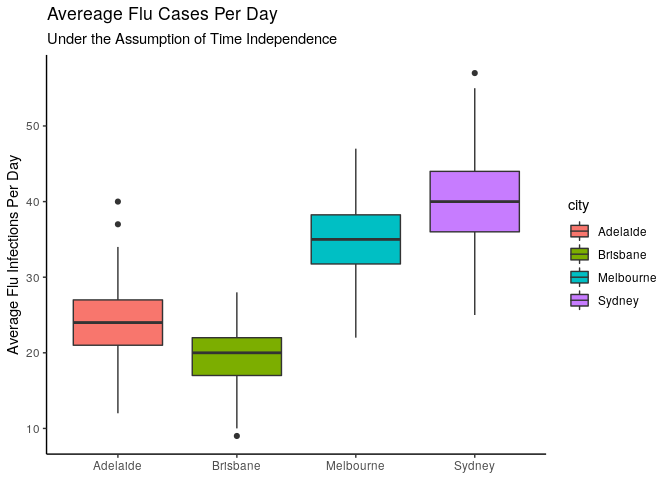
\includegraphics{main_files/figure-html/unnamed-chunk-5-1.png}

\hypertarget{observations-from-plot}{%
\subsection{Observations from Plot}\label{observations-from-plot}}

The boxplot strongly suggests that the number of infections in Sydney
and Melbourne are higher than in Adelaide or Brisbane, it would be
reasonable to expect that Sydney would have a statistically higher mean
value of new cases.

An \emph{ANOVA} test can only measure whether or not there is difference
between groups, it would be expected that this difference is
statistically signifiant.

\hypertarget{analysis-and-results}{%
\subsection{Analysis and Results}\label{analysis-and-results}}

In order to assess whether or not the mean value does differ accross
these cities a hypothesis test will be established.

\hypertarget{hypothesis}{%
\subsubsection{Hypothesis}\label{hypothesis}}

\begin{itemize}
\tightlist
\item
  \(H_0: \quad\) The mean value accross populations does not change

  \begin{itemize}
  \tightlist
  \item
    And hence we would expect the mean value to be the overall mean
  \end{itemize}
\item
  \(H_{a}: \quad\) There is a difference between the mean values across
  cities.
\end{itemize}

\hypertarget{test-statistic}{%
\subsubsection{Test statistic}\label{test-statistic}}

The \(F\) statistic is given by equation \eqref{F} and compares the
variance within groups to the variance outside groups:

\begin{align}
F &= \frac{\mathrm{SS}_B/(K-1)}{\mathrm{SS}_W(K-1)}  \label{F} \\
\ \notag \\
& \quad \qquad S S_{B}=\sum_{i=1}^{K} n_{k}\left(\bar{x}_{k}-\bar{x}\right)^{2} \label{ssb} \\
& \quad \qquad S S_{W}=\sum_{i=1}^{K}\left(n_{k}-1\right) s_{k}^{2} \label{ssw}
\end{align}

where:

\begin{itemize}
\tightlist
\item
  \(k\) is the group number or city.
\item
  \(K\) is the number of groups (In this case 4 cities)
\item
  \(SS_B\) is the sum of squared differences from the group means to the
  overall means as defined in equation \eqref{ssb}
\item
  \(SS_W\) is the sum of squared differences between group values and
  group mean as defined in equation \eqref{ssw}
\end{itemize}

The \(F\) statistic can also be calculated in \textbf{\emph{R}} using
the \passthrough{\lstinline!oneway!} function like so:

\begin{lstlisting}[language=R]
(F_obs <- oneway.test(newFlu ~ city, data, var.equal = FALSE))
\end{lstlisting}

\begin{lstlisting}
## 
##  One-way analysis of means (not assuming equal variances)
## 
## data:  newFlu and city
## F = 369.47, num df = 3.00, denom df = 217.21, p-value < 2.2e-16
\end{lstlisting}

\begin{lstlisting}[language=R]
F_obs <- F_obs$statistic
\end{lstlisting}

\hypertarget{rejection-region}{%
\subsubsection{Rejection Region}\label{rejection-region}}

Rather than using the \(F\) statistic directly, the statistic of concern
will be the probability of a Type I error (\(\alpha\)) which is
essentially a false positive.

The null hypothesis will be rejected for an \(\alpha\) value less than
5\%, this represents a low probability of a type I error which is good
evidence for rejecting the null hypothesis.

This value was reported above by the
\passthrough{\lstinline!oneway.test!} function but will be derived from
first principles below.

\hypertarget{statistic}{%
\subsubsection{Statistic}\label{statistic}}

The \(p\)-value is the measured probability of a type I error, it can be
measured by:

\begin{enumerate}
\def\labelenumi{\arabic{enumi}.}
\tightlist
\item
  Simulating the data under the assumption that the null hypothesis is
  true
\item
  Determining the frequency at which the null hypothesis would be
  rejected by mere chance

  \begin{itemize}
  \tightlist
  \item
    This frequency will be accepted as the probability of a type I
    error.
  \end{itemize}
\end{enumerate}

In order to simulate the data, the observations can be permuted in order
remove any meaningful difference between mean values that would violate
the null hypothesis and the \(F\) statistic measured. The frequency at
which a more extreme F value is observed is the \(p\) value, this is
shown below:

\begin{lstlisting}[language=R]
x <- replicate(10^3, {
  ## Permute the Categories to satisfy H_0
  city_perm <- sample(data$city)
  ## Calculate the F-Statistic
#  F_sim <- oneway.test(newFlu ~ city, data, var.equal = FALSE)$statistic

  ## Calculate Summary Statistics
  K <- length(unique(data$city))
  sd_within_groups <- aggregate(newFlu ~ city, data, sd)$newFlu^2
  xbar <- mean(data$newFlu)
  xbar_within_groups <- aggregate(newFlu ~ city, data, mean)$newFlu

  ## Calculate Squared Sums
  SSB <- length(xbar_within_groups)*(xbar_within_groups-xbar)^2
  SSW <- sum((length(sd_within_groups)-1)*sd_within_groups)

  ## Divide to get F
  F_sim <- (SSB/(K-1) ) / (SSW/(K-1))

  ## Is this more extreme than what we saw?
  F_sim > F_obs
  })

## Average the values
mean(x)
\end{lstlisting}

\begin{lstlisting}
## [1] 0
\end{lstlisting}

This returns a \(p\) -value of 0 which is consistent with the built in
output of the \passthrough{\lstinline!oneway!} function.

\hypertarget{conclusion}{%
\subsection{Conclusion}\label{conclusion}}

The probability of rejecting the null hypothesis is very small, this is
good evidence to support rejecting the null hypothesis, and because the
\(p\) value is smaller than the threshold we accept the alternative
hypothesis.

This probability does not provide us sufficient information however, to
determine the probability of correctly accepting the null hypothesis
\((1-\beta)\).

The hypothesis that the rates of infection across cities are equal
should be rejected.

\hypertarget{question-2}{%
\section{Comparison of Sydney and Melboure \normalsize \qquad ($t$-test)}\label{question-2}}

\begin{quote}
After more investigation, it was found that the sample data was
collected from the set of people who visitedthe major city hospital in
the last year. The number of people involved in the study is provided
below.Test if there is a difference in proportions of the total number
of new cases (over the 100 days) between Melbourne and Sydney.
\end{quote}

\begin{longtable}[]{@{}ll@{}}
\toprule
& Participants\tabularnewline
\midrule
\endhead
Sydney & 40, 000\tabularnewline
Melbourne & 35, 000\tabularnewline
Brisbane & 20, 000\tabularnewline
Adelaide & 25, 000\tabularnewline
\bottomrule
\end{longtable}

\hypertarget{plot-1}{%
\subsection{Plot}\label{plot-1}}

The proportion of new cases in Sydney and Melbourne may be determined by
selecting the correct variables from the data, filtering out
observations from Sydney and Melbourne and then dividing by the number
of participants:

\begin{lstlisting}[language=R]
select <- dplyr::select
filter <- dplyr::filter

tb <- table(data$city)

prop_df <-data %>%
 filter(city %in% c("Sydney", "Melbourne")) %>%
 select(city, newFlu) %>%
 mutate(newFlu = newFlu/c(rep(40000, tb["Sydney"]),
                          rep(35000, tb["Melbourne"]))
        )

aggregate(newFlu ~ city, prop_df, mean)
\end{lstlisting}

\begin{lstlisting}
##        city      newFlu
## 1 Melbourne 0.001000286
## 2    Sydney 0.001008250
\end{lstlisting}

This provies that the number of new infections per day is at a rate of
approximately 0.1\%.

From this a boxplot can be produced to compare the two proportions:

\begin{lstlisting}[language=R]
ggplot(prop_df, aes(x = city, y = newFlu, fill = city)) +
  geom_boxplot() +
  theme_bw() +
    theme(axis.title.x = element_blank()) +
  guides(fill = FALSE) +
  labs(y = "New Flu Cases Per Day", title = "Comparison of Flu Cases Against Sydney and Melbourne")
\end{lstlisting}

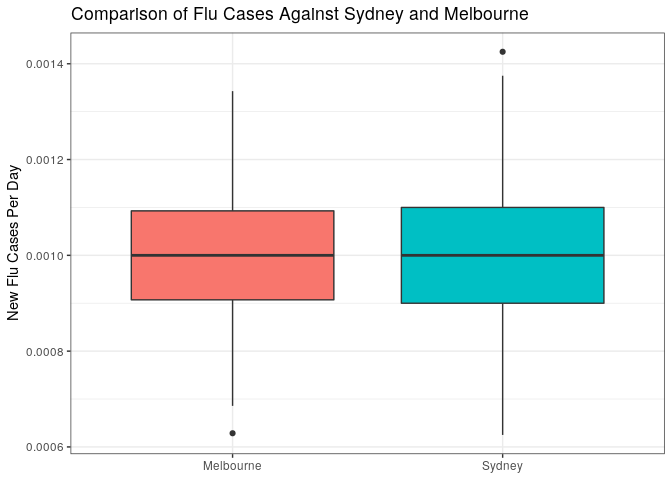
\includegraphics{main_files/figure-html/unnamed-chunk-9-1.png}

\hypertarget{observations-from-plot-1}{%
\subsection{Observations from Plot}\label{observations-from-plot-1}}

The plot does not suggest that there is any difference between the
proportion of new cases between Sydney and Melbourne.

\hypertarget{analysis-and-results-1}{%
\subsection{Analysis and Results}\label{analysis-and-results-1}}

\hypertarget{students-t-distribution}{%
\subsubsection{\texorpdfstring{Student's
\(t\)-distribution}{Student's t-distribution}}\label{students-t-distribution}}

The \emph{Central Limit Theorem} provides that the distribution of mean
values from samples of a population will be normally distributed such
that \(\overline{X} \sim \mathcal{N}\left(0, \frac{s}{\sqrt{n}}\right)\)
if:

\begin{itemize}
\tightlist
\item
  those samples are sufficiently large, or
\item
  the population is normally distributed
\end{itemize}

This means that a standardised value for the distribution of mean values
can be used to measure the \(p\)-value as shown in equation
\eqref{ttest}.

\begin{align}
z_{i}& = \frac{x_i - \overline{x}}{s}\\
& \implies  t= \frac{\left( \overline{x_1} - \overline{x_2} \right) - 0}{s_p \times \sqrt{\frac{1}{n_1} +  \frac{1}{n_2}} } \label{ttest}
\end{align}

This sample is sufficiently large and so the use of the \(t\)-test is
appropriate, this test is built into \textbf{\emph{R}} and can be
implemented with the \passthrough{\lstinline!t.test!} function:

\begin{lstlisting}[language=R]
t.test(newFlu ~ city, prop_df)
\end{lstlisting}

\begin{lstlisting}
## 
##  Welch Two Sample t-test
## 
## data:  newFlu by city
## t = -0.36942, df = 197.98, p-value = 0.7122
## alternative hypothesis: true difference in means is not equal to 0
## 95 percent confidence interval:
##  -5.047898e-05  3.455041e-05
## sample estimates:
## mean in group Melbourne    mean in group Sydney 
##             0.001000286             0.001008250
\end{lstlisting}

This provides a large \(p\)-value indicating a high probability that any
differences in the sample observations are a result of mere chance
rather than indicative of a difference in population means.

\hypertarget{simulation}{%
\subsubsection{Simulation}\label{simulation}}

This test can also be performed by simulation by:

\begin{enumerate}
\def\labelenumi{\arabic{enumi}.}
\tightlist
\item
  Assuming that there is no difference in the data
\item
  Permuting the city to which the value corresponds in order remove any
  difference
\item
  measuring the difference between the average of the two cities
\item
  repeating this many times
\end{enumerate}

The frequency at which a difference more extreme that what was observed
is detected is a measurement of the probability of committing a type I
error under the assumption that the null hypothesis is true, this is the
\(p\)-value.

\begin{lstlisting}[language=R]
set.seed(85284)

mean_diff_obs <- aggregate(newFlu ~ city, prop_df, mean)[,2] %>% diff()

xbar_sim <- replicate(10^3, {
  city_perm <- sample(prop_df$city)
  mean_diff_sim <- aggregate(newFlu ~ city_perm, prop_df, mean)[,2] %>% diff()

  # Is this more extreme? Is it a false pos?
  abs(mean_diff_sim) > abs(mean_diff_obs)
})

# What Proportion are false postive?
mean(xbar_sim)
\end{lstlisting}

\begin{lstlisting}
## [1] 0.719
\end{lstlisting}

This shows, assuming there is no difference between the two populations,
that the probability of detecting such a change is \(\approx 72\%\),
this is consistent with the \(t\)-test from before.

\hypertarget{conclusion-1}{%
\subsection{Conclusion}\label{conclusion-1}}

A \(p\)-value in excess of 0.7 is very large and indicates that there is
insufficient evidence to reject the hypothesis that there is a
difference between the mean value of the proportion of new infections
between cities.

Hence it is \emph{not} concluded that there is any difference.

\hypertarget{question-3}{%
\section{Correlation of Sydney and Adelaide \normalsize \qquad (\texttt{bootstrap})}\label{question-3}}

\begin{quote}
The recent trend of people from Sydney spending their vacations in
Adelaide has lead to the belief that the trends in the tiara virus are
related. Compute the confidence interval for the correlation of new
cases of tiara virus between Sydney and Adelaide.
\end{quote}

\hypertarget{plot-2}{%
\subsection{Plot}\label{plot-2}}

In order to assess the correlation between case rates across the two
cities it is necessary to first pivot the data frame into a different
format. This can by done by using \passthrough{\lstinline!dplyr!} to
select the appropriate features, filter based on the city and then
transform the data into a wide format like so:

\begin{lstlisting}[language=R]
(cor_df <- data %>%
  group_by(city) %>%
  select(city, newTiara, date) %>%
  filter(city %in% c("Sydney", "Adelaide")) %>%
  pivot_wider(names_from = city, values_from = newTiara) ) %>% head()
\end{lstlisting}

\begin{lstlisting}
## # A tibble: 6 x 3
##    date Sydney Adelaide
##   <int>  <int>    <int>
## 1     1      1      106
## 2     2      2       48
## 3     3      4       99
## 4     4      0       92
## 5     5      3       63
## 6     6      4       73
\end{lstlisting}

This data can then be used to produce a scatter plot comparing the two
rates:

\begin{lstlisting}[language=R]
ggplot(cor_df, aes(x = Sydney, y = Adelaide)) +
  geom_point(aes(col = date)) +
  stat_smooth(method = 'lm', lty = 3) +
  theme_classic() +
  labs(title = "Comparison of New Tiara Cases across Sydney and Adelaide") +
   guides(col = guide_legend("Days Since \nFirst Case"))
\end{lstlisting}

\begin{lstlisting}
## `geom_smooth()` using formula 'y ~ x'
\end{lstlisting}

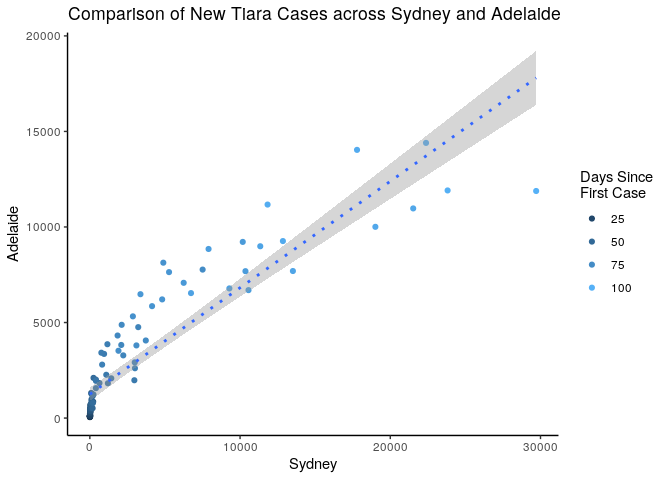
\includegraphics{main_files/figure-html/unnamed-chunk-13-1.png}

\hypertarget{observations-from-plot-2}{%
\subsection{Observations from Plot}\label{observations-from-plot-2}}

This plot suggests that there is a significant amount of correlation
between the two variables. The relationship is a monotone positive one
but it is non-linear and likely logarithmic.

\hypertarget{analysis-and-results-2}{%
\subsection{Analysis and Results}\label{analysis-and-results-2}}

In order to create a confidence interval of the data a boot strap
simulation can be used:

\begin{enumerate}
\def\labelenumi{\arabic{enumi}.}
\tightlist
\item
  Assume that the population is an infinite repetition of the sample
\item
  Take a sample from this population

  \begin{itemize}
  \tightlist
  \item
    This can be acheived by resampling the sample with repetition.
  \end{itemize}
\item
  compute the correlation and repeat.
\end{enumerate}

This will give a normally distributed range of values for the
correlation coefficient (\(\rho\)). This distribution can be used to
estimate the range of \(\rho\) values for samples drawn from the
population by taking the quantiles, this represents an estimate for the
confidence interval.

The confidence interval is a measure of the probability that any given
sample from a population will contain the population mean, for example,
a 95\% confidence interval of some sample from a population will have a
95\% probability of containing the population mean. In saying that
however, that does not imply that there is a 95\% probability of this
confidence interval containing the population mean, \(\mu\) is not a
random variable and so it's not correct to talk about probabilities,
rather it is expressed that there is a 95\% confidence level that the
the population mean is contained in that interval.

A 95\% confidence interval of the correlation coefficient can be
produced via the bootstrap approach:

\begin{lstlisting}[language=R]
n <- nrow(cor_df)

sim <- replicate(10^3, {
    index <- sample(1:n, size = n, replace = TRUE)
    df    <- cor_df[index,]
    cor(df[,1], df[,2])
})
quantile(sim, c(0.025, 0.0975))
\end{lstlisting}

\begin{lstlisting}
##      2.5%     9.75% 
## 0.6680477 0.6835098
\end{lstlisting}

This provides that a 95\% confidence interval for the correlation
coefficient is \(\rho \in \left(0.668, 0.684\right)\)

\hypertarget{conclusion-2}{%
\subsection{Conclusion}\label{conclusion-2}}

The 95\% confidence interval for the correlation coefficient provides a
range of values that is reasonably large, hence it may be concluded with
a high degree of certainty that there is a \textbf{moderate} amount of
correlation for the number of new cases of \emph{Tiaria} between Sydney
and Adelaide.

\hypertarget{question-4}{%
\section{Rate of Change in Sydney \qquad \normalsize(\texttt{bootstrap}; \textit{Least-Squares Regression})}\label{question-4}}

\begin{quote}
A colleague has observed that the daily new infections of the Tiara
virus seem to increase exponentially with time, implying a relationship:
\[
y = Ae^{\beta x} \\
\] where x is the date, and y is the number of new infections. Using a
log transformation changes the model to: \[
\log{\left(y\right)} = \log{\left(A\right)} + \beta x
\] which is now a linear model.

Compute the confidence interval for the parameter \(\beta\) for the new
infections in Sydney.
\end{quote}

\hypertarget{plot-3}{%
\subsection{Plot}\label{plot-3}}

In order to produce a plot of the data it is necessary to produce a
corresponding data frame. The \passthrough{\lstinline!dplyr!} package
can be used to \passthrough{\lstinline!select!} the appropriate features
and then \passthrough{\lstinline!ggplot!} can be used to produce a plot
and a \(\log\)-transformed plot:

\begin{lstlisting}[language=R]
p_raw <- ggplot(data, aes(x = date, y = newTiara, col = city)) +
  geom_point() +
  theme_classic() +
  labs(x = "Days Since First Case",
       y = "Number of New Tiara Cases",
       title = "New Tiara Cases") +
  theme(legend.position = c(0.3, 0.7)) +
  guides(col = guide_legend("City")) +
  theme(legend.background = element_rect(fill="#f0f0f0",
                                  size=0.6, linetype="solid",
                                  colour ="darkblue"))


# No need to clean out x<1 with ggplot2
# data[(data$newTiara<1),]

p_log_trans <- ggplot(data, aes(x = log(date), y = log(newTiara), col = city)) +
  geom_point(alpha = 0.7) +
  stat_smooth(method = 'lm', se = TRUE) +
#  stat_smooth(lty = 3, se = FALSE) +
  scale_y_continuous(limits = c(0, 10)) +
  scale_x_continuous(limits = c(0, log(max(data$date)))) +
  theme_classic() +
  guides(col = FALSE) +
  labs(x = "Natural log of Days Since First Case",
       y = "Number of New Tiara Cases",
       title = "New Tiara Cases, Log Transform",
         subtitle = "Using the natural log")


library(gridExtra)
grid.arrange(grobs = list(p_raw, p_log_trans), layout_matrix = matrix(1:2, nrow = 1))
\end{lstlisting}

\begin{lstlisting}
## `geom_smooth()` using formula 'y ~ x'
\end{lstlisting}

\begin{lstlisting}
## Warning: Removed 20 rows containing non-finite values (stat_smooth).
\end{lstlisting}

\begin{lstlisting}
## Warning: Removed 4 rows containing missing values (geom_point).
\end{lstlisting}

\begin{lstlisting}
## Warning: Removed 71 rows containing missing values (geom_smooth).
\end{lstlisting}

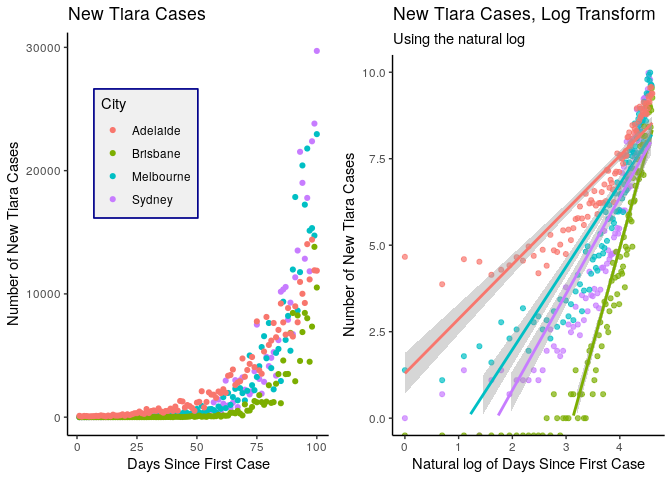
\includegraphics{main_files/figure-html/unnamed-chunk-15-1.png}

\hypertarget{observations-from-plot-3}{%
\subsection{Observations from Plot}\label{observations-from-plot-3}}

Following the transform the data is quite linear and this, in conjuction
with mathematical reasoning, is good evidence to justify the use of an
exponential model, there does however appear to be a slight non linear
trend in the data corresponding to Adelaide following the transform.

Looking at the plot and taking the rise over run, the \(\beta\)
coefficient would appear to be about
\(\beta \approx \frac{7.5-0}{4-1} = 2.5\).

\hypertarget{analysis-and-results-3}{%
\subsection{Analysis and Results}\label{analysis-and-results-3}}

In order to produce a confidence interval for the slope of the log
transformed data it is necessary to first produce a corresponding data
frame, this can be acheived by using \passthrough{\lstinline!dplyr!} to
select the appropriate features, mutate the values and filter out any
\(-\infty\) values:

\begin{lstlisting}[language=R]
(log_trans <- data %>%
  select(city, newTiara, date) %>%
   filter(city == "Sydney") %>%
  mutate(newTiara = log(newTiara),
         date     = log(date)) %>%
  filter(newTiara != -Inf )) %>%
  head()
\end{lstlisting}

\begin{lstlisting}
##     city  newTiara      date
## 1 Sydney 0.0000000 0.0000000
## 2 Sydney 0.6931472 0.6931472
## 3 Sydney 1.3862944 1.0986123
## 4 Sydney 1.0986123 1.6094379
## 5 Sydney 1.3862944 1.7917595
## 6 Sydney 0.6931472 1.9459101
\end{lstlisting}

To produce a confidence interval for the slope value:

\begin{enumerate}
\def\labelenumi{\arabic{enumi}.}
\tightlist
\item
  Assume that the population is composed of an infinite repetition of
  the sample
\item
  Sample from this broader population (by resampling with repetition)
\item
  Calculate the slope value
\item
  repeat many times in order to produce a distribution
\end{enumerate}

The quantile of the distribution is hence given by:

\begin{lstlisting}[language=R]
n = nrow(log_trans)

beta = replicate(1000, {
## Resample the Data
samp = sample(1:n, replace = TRUE, size = n) # sample the row numbers (with replacement)

## Fit the Regression
fit = lm(newTiara ~ date, data = log_trans[samp,])

## Extract the Slope
coef(fit)[2] # extract the estimate of b
})
## print out the interval boundaries (95% interval)
(limits <- quantile(beta, c(0.025, 0.975)))
\end{lstlisting}

\begin{lstlisting}
##   2.5%    97.5%
## 2.403382 3.702158
\end{lstlisting}

This boot strap distribution can be visualised using a histogram:

\begin{lstlisting}[language=R]
ggplot(tibble::enframe(beta), aes(x = value, y = after_stat(density))) +
  geom_histogram(fill = "LightSkyBlue", col = "purple", bins = 20) +
  geom_vline(xintercept = limits[1]) +
  geom_vline(xintercept = limits[2]) +
  theme_bw() +
  labs(x = latex2exp::TeX('Bootstrapped $\\beta$ Coefficient'),
       subtitle = "Regressed from log transform using least squares", 
       main = "Distribution of exponential coefficient", 
       y = "Density")
\end{lstlisting}

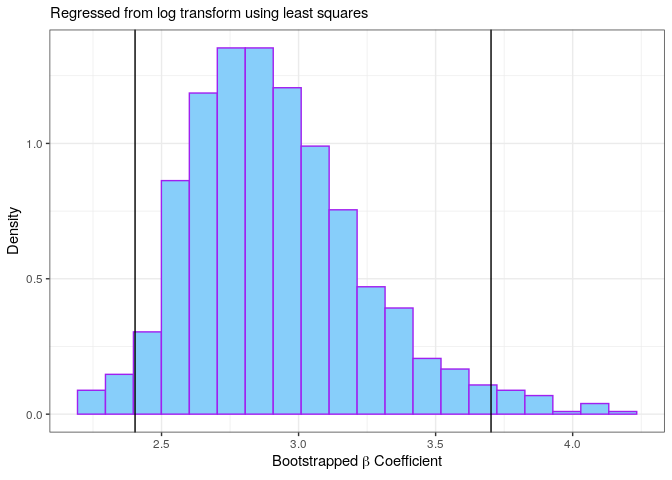
\includegraphics{main_files/figure-html/unnamed-chunk-18-1.png} \#\#
Conclusion The bootstrap provides that a 95\% confidence interval for
\(\beta\) is between 2.4 and 3.7, this is a good estimate for the rate at
which the average number of transmissions per person changes (i.e.~the
acceleration of the spread or the second derivative of the number of
infected). \#\#\# Note on Log Transforms It's worth acknowledging that
the slope coefficient of the log-transformed data does not solve the
least squares optimisation problem for an exponential model, this would
require a numerical solution (which would be too slow to bootstrap) and
so this is appropriate estimation.

\hypertarget{question-5}{%
\section{Comparison of Sydney and Melbourne Rates \normalsize \qquad (\texttt{bootstrap})}\label{question-5}}

\begin{quote}
The final piece of analysis wanted by the health minister is to
determine if the Tiara virus is spreading at a slower rate in Melbourne
when compared to Sydney. Perform a hypothesis test to test if the rate
of increase of new Tiara virus cases b is lower in Melbourne when
compared to Sydney.
\end{quote}

\hypertarget{plot-4}{%
\subsection{Plot}\label{plot-4}}

In order to plot the data it is necessary to filter the results for
Sydney and Melbourne, this can be done using
\passthrough{\lstinline!dplyr!}. This data is best described by an
exponential model as justified by equation \eqref{expmod} and so the
rate considered should be the rate coefficient (\(\beta\)) in the
expoential model.

In order to justify the expoenential model let \(p\) be the number of
people with the disease, we would expect the growth of this population
to be proportional to the number of those infected:

\begin{align}
p &\propto \frac{\mathrm{d}p}{\mathrm{d}t} \notag \\
\implies \int  \enspace \mathrm{d}t &\propto \int \frac{1}{p} \frac{\mathrm{d}p}{\mathrm{d}t} \enspace \mathrm{d}t \notag \\
\text{using integration by parts:} \notag \\
\implies \int  \enspace \mathrm{d}t &\propto \int \frac{1}{p} \enspace \mathrm{d}t \notag \\
 t &\propto \ln{\mid p \mid } + C, \quad \exists C \in \mathbb{R} \notag \\
 p \text{ is always positve and so } \mid p \mid \propto p: \notag \\
 t &\propto \ln{ p  } + C, \quad \exists C \in \mathbb{R} \notag \\
 \text{provide proportionality constant:} \notag \\
 e^{\beta t} &= e^{\ln{ p  } + C}, \quad \exists \beta, C \in \mathbb{R}\notag \\
 \implies p &= \gamma e^{\beta t}, \exists \beta, C \in \mathbb{R} \\
\frac{\mathrm{d}p}{\mathrm{d}t} &= \alpha e^{\beta t}, \exists \beta, C \in \mathbb{R}\label{expmod} \\
\end{align}

\(\therefore\) the rate of change of new cases, assuming that the rate
of spread is proportional to the number of infected, would be described
by an exponential model.

Plots can be produces in a similar fashion as the before in order to
illustrate the difference in rates:

\begin{lstlisting}[language=R]
syd_mel_data <- data %>% 
  filter(city %in% c("Sydney", "Melbourne"))

p_raw <- ggplot(syd_mel_data, aes(x = date, y = newTiara, col = city)) +
  geom_point() +
  theme_classic() +
  labs(x = "Days Since First Case",
       y = "Number of New Tiara Cases",
       title = "Melbourne and Sydney, Daily Tiara Cases, Log Transform") +
  theme(legend.position = c(0.3, 0.7)) +
  guides(col = guide_legend("City")) +
  theme(legend.background = element_rect(fill="#f0f0f0",
                                  size=0.6, linetype="solid",
                                  colour ="darkblue"))

p_log_trans <- ggplot(syd_mel_data, aes(x = log(date), y = log(newTiara), col = city)) +
  geom_point(alpha = 0.7) +
  stat_smooth(method = 'lm', se = TRUE) +
  scale_y_continuous(limits = c(0, 10)) +
  scale_x_continuous(limits = c(0, log(max(data$date)))) +
  theme_classic() +
  guides(col = FALSE) +
  labs(x = "Natural log of Days Since First Case",
       y = "Number of New Tiara Cases",
       title = "Melbourne and Sydney, Daily Tiara Cases, Log Transform",
         subtitle = "Using the natural log")


library(gridExtra)
grid.arrange(grobs = list(p_raw, p_log_trans), layout_matrix = matrix(1:2, nrow = 1))
\end{lstlisting}

\begin{lstlisting}
## `geom_smooth()` using formula 'y ~ x'
\end{lstlisting}

\begin{lstlisting}
## Warning: Removed 5 rows containing non-finite values (stat_smooth).
\end{lstlisting}

\begin{lstlisting}
## Warning: Removed 4 rows containing missing values (geom_point).
\end{lstlisting}

\begin{lstlisting}
## Warning: Removed 51 rows containing missing values (geom_smooth).
\end{lstlisting}

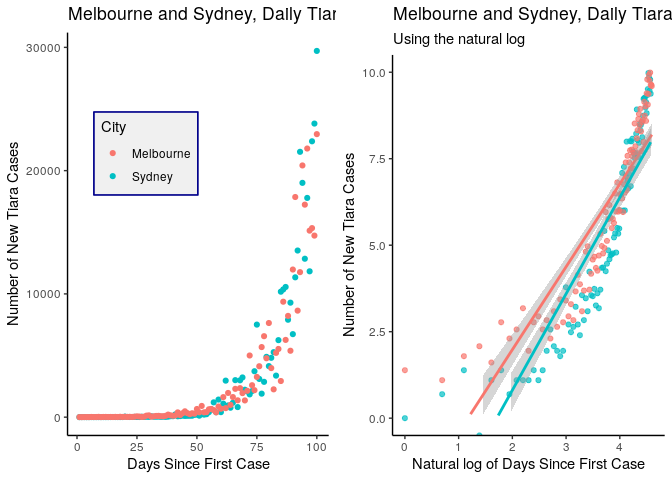
\includegraphics{main_files/figure-html/unnamed-chunk-19-1.png}

\hypertarget{observations-from-plot-4}{%
\subsection{Observations from Plot}\label{observations-from-plot-4}}

The plot suggests that Melbourne has a higher number of new daily cases
of \emph{Tiara} Virus, the rate of increase of new cases in Sydney does
however appear significantly (albeit slightly) greater than Melbourne.

It appears that Sydney has a higher rate of new coronavirus cases.

\hypertarget{analysis-and-results-4}{%
\subsection{Analysis and Results}\label{analysis-and-results-4}}

In order to consider the rate of change of new cases of \emph{Tiara}
virus the data must be filtered for results only pertaining to Sydney
and Melbourne and pivoted into a longer format, this can be done with
\passthrough{\lstinline!dplyr!}:

\begin{lstlisting}[language=R]
## Relevant data
rate_df <- data %>% 
  ## Throw away other features
  select(city, newTiara, date) %>% 
  ## Only use Melbourne and Sydney
  filter(city %in% c("Sydney", "Melbourne")) %>% 
  ## Tage out zero values for the log transform
  filter(newTiara > 0) %>% 
  ## Make the DataFrame wider
  pivot_wider(names_from = city, values_from = newTiara)
\end{lstlisting}

Then that data can be used to compare the slope of the log transformed
data between the two cities:

\begin{lstlisting}[language=R]
## Calculate the slope
rate_diff <- function(data) {
  
sydney_mod <- lm(log(Sydney) ~ log(date), data)
sydney_slope <- sydney_mod$coefficients[2]

melbourne_mod <- lm(log(Melbourne) ~ log(date), data)
melbourne_slope <- melbourne_mod$coefficients[2]

(slope_diff <- sydney_slope-melbourne_slope)
}

(slope_diff_obs <- rate_diff(rate_df))
\end{lstlisting}

\begin{lstlisting}
## log(date) 
##  0.442499
\end{lstlisting}

This suggests that the rate of new cases in Sydney is higher than
Melbourne, by a rate of about 0.44.

\hypertarget{hypothesis-1}{%
\subsubsection{Hypothesis}\label{hypothesis-1}}

In order to perform a hypothesis test it is necessary to stipulate two
hypothesis:

\begin{enumerate}
\def\labelenumi{\arabic{enumi}.}
\tightlist
\item
  \(H_0: \quad\) The rate of change of daily new cases is equal in
  Sydney and Melbourne.

  \begin{itemize}
  \tightlist
  \item
    \(\beta_\mathrm{Syd} - \beta_\mathrm{Mel} = 0\)
  \end{itemize}
\item
  \(H_a: \quad\) Sydney has a higher rate of new daily cases than
  Melbourne.

  \begin{itemize}
  \tightlist
  \item
    \(\beta_\mathrm{Syd} - \beta_\mathrm{Mel} > 0\)
  \end{itemize}
\end{enumerate}

\hypertarget{test-statistic-1}{%
\subsubsection{Test Statistic}\label{test-statistic-1}}

In order to measure the \(p\) value the data needs to be simulated under
the assumption that the null hypothesis is true, the frequency at which
the difference between the slope values is atleast as great as the
observation is a good estimate for the probability of committing a type
I error, this is the \(p\) value. A low \(p\)-value is good evidence to
support rejecting the null hypothesis.

To simulate the null hypothesis, combine the observations and randomly
assign them to either city, the \(\beta\) values can then be measured,
differenced and recorded like so:

\begin{lstlisting}[language=R]
##H0 is that the b_0-b1 = 0

start <- Sys.time()
sim_diff_vec <- replicate(10^3, {
## Combine the cities and randomly permut the cases between
   (rate_df_perm <- data %>% 
     group_by(date) %>% 
     select(city, newTiara, date) %>% 
     filter(city %in% c("Sydney", "Melbourne")) %>% 
     mutate(city = sample(city)) %>% 
     filter(newTiara > 0) %>% 
     pivot_wider(names_from = city, values_from = newTiara))
  
## Calculate the slope
sim_diff <- rate_diff(rate_df_perm)

return(sim_diff)
}) 

## Is this difference greater than the observation?
fpos <-  (sim_diff_vec > slope_diff_obs)

(p <- mean(fpos))
\end{lstlisting}

\begin{lstlisting}
## [1] 0
\end{lstlisting}

\begin{lstlisting}[language=R]
Sys.time()-start
\end{lstlisting}

\begin{lstlisting}
## Time difference of 36.59436 secs
\end{lstlisting}

This distribution can be plotted as a histogram in order to visualise
the significance of the difference in rates:

\begin{lstlisting}[language=R]
ggplot(tibble::enframe(sim_diff_vec), aes(x = value, y = after_stat(density))) +
  geom_histogram(fill = "LightSkyBlue", col = "purple", bins = 20) +
  geom_vline(xintercept = slope_diff_obs, lty = 2, col = "purple") +
  theme_bw() +
  labs(x = latex2exp::TeX('Difference in $\\beta$ Coefficient values'),
       subtitle = "Regressed from log transform using least squares", 
       main = "Distribution of Difference in new case rates between Sydney and Melbourne", 
       y = "Density")
\end{lstlisting}

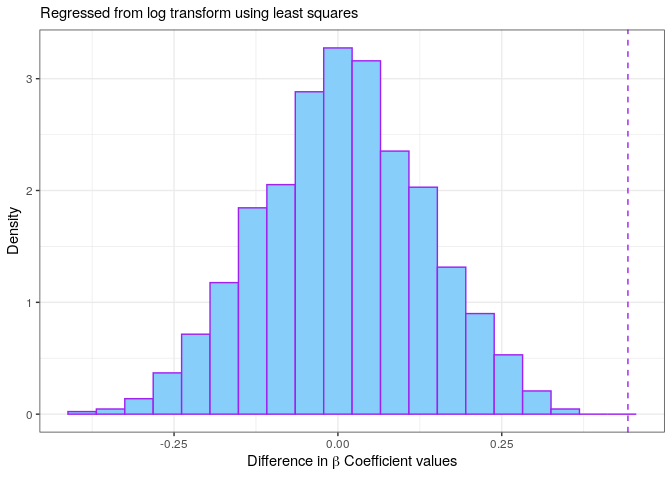
\includegraphics{main_files/figure-html/unnamed-chunk-23-1.png}

\hypertarget{conclusion-3}{%
\subsection{Conclusion}\label{conclusion-3}}

Under the assumption that the rates of daily new cases are equivalent,
the probability of detecting a difference when there was none is
practically 0, this is good evidence to support rejecting the null
hypothesis.

It is hence concluded that there is sufficient evidence to reject the
hypothesis that the rate of change of cases is lower in Sydney than
Melbourne.

\end{document}
